\section{Data and Results}
Five experiments were performed using a constant amount of carbonic anhydrase and varying concentrations of dipic. For each experiment, several measurements of CA-catalyzed pNPA hydrolysis velocities, $ln \left(\frac{dA}{dt}\right)_{cat}$, were taken using spectrophotometry and plotted against the CA/dipic reaction time. The results of these experiments are shown in Figure \ref{fig:kobs_results}.
\begin{figure}[h]
        \begin{subfigure}{0.5\textwidth}
                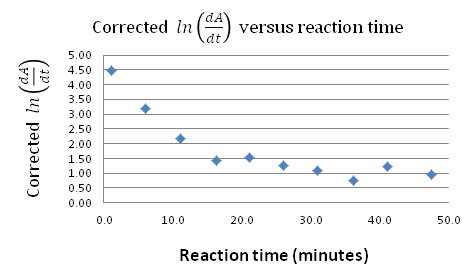
\includegraphics[width=\textwidth]{./Figures/20M_dipic_readings.png}
                \caption{0.20 M dipic}
                \label{fig:0.20M_dipic_readings}
        \end{subfigure}\begin{subfigure}{0.5\textwidth}
                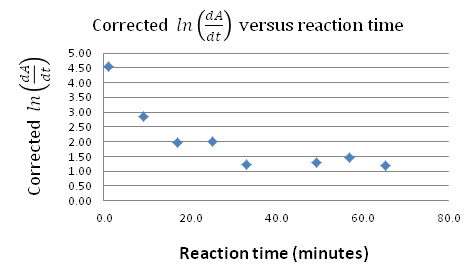
\includegraphics[width=\textwidth]{./Figures/10M_dipic_readings.png}
                \caption{0.10 M dipic}
                \label{fig:0.10M_dipic_readings}
        \end{subfigure}
        \begin{subfigure}{0.5\textwidth}
                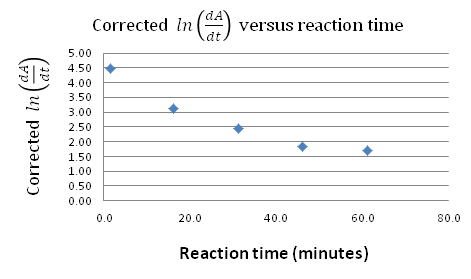
\includegraphics[width=\textwidth]{./Figures/05M_dipic_readings.png}
                \caption{0.05 M dipic}
                \label{fig:0.05M_dipic_readings}
        \end{subfigure}\begin{subfigure}{0.5\textwidth}
                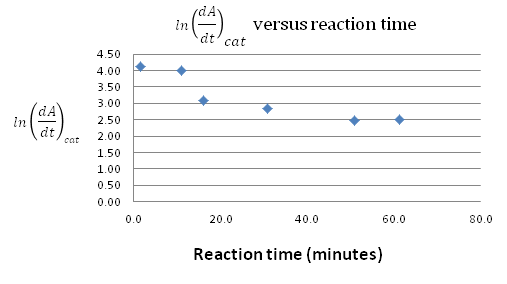
\includegraphics[width=\textwidth]{./Figures/032M_dipic_readings.png}
                \caption{0.032 M dipic}
                \label{fig:0.032M_dipic_readings}
        \end{subfigure}
        \begin{subfigure}{0.5\textwidth}
                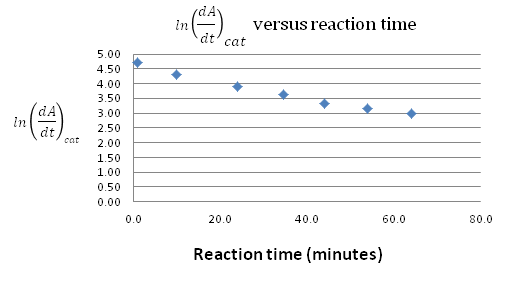
\includegraphics[width=\textwidth]{./Figures/016M_dipic_readings.png}
                \caption{0.016 M dipic}
                \label{fig:0.016M_dipic_readings}
        \end{subfigure}
        \caption{$ln \left(\frac{dA}{dt}\right)_{cat}$ measurements versus CA/dipic reaction time for various concentrations of dipic. Slopes of the descending portions of these plots were used to assign values for $k_{obs}$.}\label{fig:kobs_results}
\end{figure}

From the descending portions of the plots shown in Figure \ref{fig:kobs_results}, five values of $k_{obs}$ were calculated using the slopes determined by least squares regression. The reciprocals of $k_{obs}$ and $\text{[L]}_0$ (dipic concentration) were plotted against each other, as shown in Figure \ref{fig:kobs_vs_l}.

\begin{figure}[h]
  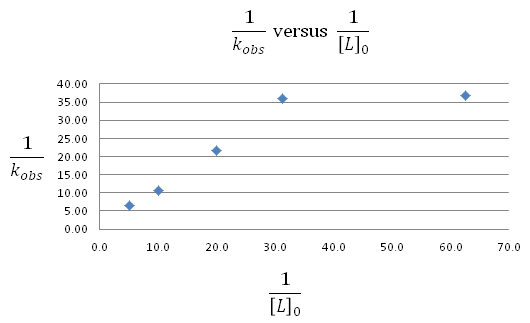
\includegraphics[scale=.5]{./Figures/kobs_vs_l.png}\\
  \caption{Plot of $\frac{1}{k_{obs}}$ versus $\frac{1}{\text{[L]}_0}$. The slope and intercept of the line passing through these points were determined by least squares regression and used to calculate $K_{EML}$ and $k_d$, demonstrated by Equations \eqref{eqn:samp_calc_keml} and \eqref{eqn:samp_calc_kd} respectively.}\label{fig:kobs_vs_l}
\end{figure}

A least squares regression procedure was performed on the data shown in Figure \ref{fig:kobs_vs_l} to retrieve values for the slope and intercept of the line passing through those points. Equations \eqref{eqn:samp_calc_keml} and \eqref{eqn:samp_calc_kd} show how these were used to calculate $K_{EML}$ and $k_d$. Table \ref{tbl:summary} lists these values and their 95\% confidence intervals, as well as accepted values reported in literature.

\begin{table}[h]
    \begin{tabular}{| l | l | l |}
    \hline
    Constant & Empirical Value & Accepted Value \\ \hline
    $K_{EML}$ & $(20\pm{18}){\ }M^{-1}$ & $(7.7\pm{1.5}){\ }M^{-1}$ \cite{bib:easy_peasy_values} \\ \hline
    $k_{d}$ & $(0.10\pm{0.10}){\ }mins^{-1}$ & $(0.43\pm{0.08}){\ }mins^{-1}$ \cite{bib:easy_peasy_values} \\ 
    \hline
    \end{tabular}
    \caption[Table caption text]{Values of $K_{EML}$ and $k_d$, as determined in this experiment as well as accepted values from literature}
    \label{tbl:summary}
\end{table}